\documentclass[conference]{IEEEtran}
\usepackage{cancel}
\usepackage{amsmath}
\usepackage{url}
\usepackage{listings}
\usepackage{color}

% the following tells mathastext to use typewriter
\usepackage[T1]{fontenc}
\usepackage{mathastext}
\MTfamily{\ttdefault}\Mathastext 

\usepackage{bussproofs}
\usepackage[]{algorithm2e}
\usepackage{soul}
\usepackage{cancel}
\usepackage{multirow}

\input{macros}
\newsavebox{\fmbox}
\newenvironment{smpage}[1]
{\begin{lrbox}{\fmbox}\begin{minipage}{#1}}
{\end{minipage}\end{lrbox}\usebox{\fmbox}}


%\theoremstyle{definition}
\newtheorem{definition}{Definition}
\newtheorem{decision}{Requirement}
\newtheorem{law}{Requirement}
\lstset{
  basicstyle = \footnotesize\tt,
  }



\begin{document}

\title{Bidirectinalizing the C Preprocessor}

\author{
   \IEEEauthorblockN{
  Yingfei Xiong$^{1,2}$, Zhengkai Wu$^{1,2}$, Yiming Wu$^{1,2}$, Meng
  Wang$^3$, Lu Zhang$^{1,2}$}\\
\IEEEauthorblockA{$^1$Key Laboratory of High Confidence Software
  Technologies (Peking University), MoE \\$^2$Institute of Software,
  School of EECS, Peking
  University, China\\ $^3$School of Computing, University of Kent, UK}
  \IEEEauthorblockA{\{xiongyf, 1200012746, yiming.wu, zhanglucs\}@pku.edu.cn, m.w.wang@kent.ac.uk}
}

\maketitle
\begin{abstract}
  % Many programming tools work directly on source code. A typical example is a bug-fixing tool, which modifies source code to remove certain bugs in the code. With these tools, a program is first analyzed, and a change to the program is then recommended and applied to the code. We call these tools {\em program-editing tools}.

  % On the other hand, a lot of programming languages rely on preprocessors. One of the most widely-used preprocessors is the C preprocessor---formally used in C, C++, and Objective-C, and also casually by developers in other languages. In these cases, any tool that changes the source code will have to handle the preprocessor directives, which is not an easy task. Given the complexity of preprocessors, many tools either fail to produce sound results, or give up completely and deal only with preprocessed code.

  Many tools directly change programs, such as bug-fixing tools, program migration tools, etc. We call them \emph{program-editing tools}. On the other hand, many programing use the C preprocessor, such as C, C++, and Objective-C. Because of the complexity of preprocessors, many program-editing tools either fail to produce sound results under the presence of preprocessor directives, or give up completely and deal only with preprocessed code.
  
  In this paper we propose a lightweight approach that enables program-editing tools to work with the C preprocessor for (almost) free. The idea is that program-editing tools now simply target the preprocessed code, and our system, acting as a bidirectional C preprocessor, automatically propagates the changes on the preprocessed code back to the unpreprocessed code. The resulting source code is guaranteed to be correct and is kept similar to the original source as much as possible. We have evaluated our approach on Linux kernel with a set of generated changes. The evaluation results show the feasibility and effectiveness of our approach.
\end{abstract}

\section{Introduction}
\label{sec:intro}

% \begin{itemize}
% \item program editing tools
% \item preprocessors
%   \begin{itemize}
%   \item used by mainstream languages, including OO language C++ and
%     ObjectiveC
%   \item casual uses
%   \end{itemize}
% \item program editing tools meet preprocessors
% \item reality: program editing tools do not support preprocessors
% \item existing work: C preprocessor in refactoring
%   \begin{itemize}
%   \item too complicated
%   \item not general solution
%   \end{itemize}
% \item contributions
% \item outline of the paper
% \end{itemize}

A lot of program analysis tools involve direct modification of
source code. A notable category of such tools is program-repair tools
~\cite{le2012genprog,le2012systematic,QiMLDW14,nguyen2013semfix}. These tools take a program and a set of tests as
input, and
modify the program until all tests pass. Another
category is API evolution tools~\cite{li2015swin,Padioleau06,Meng:2011}.
When an API is upgraded with incompatible changes, 
these tools automatically change the API
invocations to comply with the new API. 
We call such tools that directly modify the source code 
\emph{program-editing tools}.

On the other hand, many programming languages are provided with
preprocessors~\cite{ernst2002empirical,kohlbecker1986hygienic,lee2012marco}. The most
widely used preprocessor is the C preprocessor (CPP). Many programming
languages adopt CPP, notable C, C++, and
Objective-C. Furthermore, CPP is often used by
programmers in casual situations as a general purpose tool, 
where the preprocessor is added as a
building step for any language used. For example, Korpela~\cite{Korpela2000} describes the
use CPP as an HTML authoring tool:
instead of writing HTML pages directly, the shared code pieces between HTML
pages are first defined as C macros, and HTML pages using these
macros are preprocessed into final HTML files.

Program editing tools usually do not directly change preprocessor directives. However the tools must be able to map results back to the unpreprocessed source to be useful. There is no point of fixing a bug in the preprocessed code and only to have it overwritten when the unchanged source is compiled again. This is challenging, as the tools must be able to understand both the preprocessor directives and the target programming languages, and make sure whatever changes made on both levels are consistent with each other. As a matter of fact, existing program-editing tools often fail to produce correct results under the presence of preprocessor directives, or give up dealing with them entirely. We have
investigated the implementations of three influential bug-fixing tools
on the C programming language: GenProg~\cite{le2012genprog,le2012systematic}, RSRepair~\cite{QiMLDW14}, and
SemFix~\cite{nguyen2013semfix}. All the three implementations work only on
preprocessed code. Users have to manually inspect the
preprocessed code, and copy the changes to the original source code---risking of introducing new bugs in the process. 

A closely related area is refactoring~\cite{McCloskey:2005,Garrido2013}, where tools are expected to directly manipulate preprocessor directives. For example, one may well want to rename a macro or extract a macro as part of the refactoring. In this case, tool builders have no choice but to bite the bullet and confront the preprocessor directly. 
    Typically a new C grammar is designed such that it
incorporates both the original C grammar and the preprocessor
directives. 
%This design is originated from the need of 
%refactoring tools to directly manipulate preprocessor directives,
%e.g., renaming macros. 
However, when applied to a more wider range of
code editing tools, such almost brute force approaches exhibit obvious shortcomings.
First, tool developers using such a grammar basically have to start from scratch: 
they have to learn the new grammar and leave behind the existing tool
chains on C. Second, the effort spend on the new grammars is specialized and
cannot be reused for other languages, which basically rules out  casual uses of CPP. 

In this paper we propose a lightweight approach to support
CPP in program-editing tools. Our system acts as a
bidirectional CPP: the original preprocessing can be
considered as a forward program transformation, and we add to it a corresponding 
backward transformation that maps changes on the preprocessed
code back into the unpreprocessed source. As a result, program-editing tools can now focus on preprocessed programs, and have results (almost) automatically reflected to the source\footnote{It is not entirely automatic because the tools need to support the extraction of the changes on the preprocessed programs. Although this step can be performed by generic code differencing~\cite{fluri2007change}, extracting the changes directly from the tools gives the best
result.}.



%This idea is
%based on the observation that, unlike refactoring tools that often
%have to directly manipulate the preprocessor directives, many
%program-editing tools are not directly related to preprocessor
%directives and can be implemented more conveniently with only
%preprocessed programs.
We list a few examples here: (1) as mentioned 
above the implementations of the three state-of-the-art
bug-fixing approaches only deal with preprocessed code; (2) the API
evolution tools mentioned previously can also be implemented more
conveniently by only dealing with preprocessed code; (3) all
program-editing tools on languages that do not formally rely on CPP
naturally fall into this category because the programs may be put
under casual uses of CPP.

%It is not easy to bidirectionalize CPP. 
Although there exist several
bidirectionalization
techniques~\cite{MaHNHT07,Voigtlander09bff,voigtlander2010combining},
they are designed for data transformation: given a source data set
$s$, a transformation program $p$, and a target data set $t=p(s)$,
these approaches try to reflect the changes on $t$ to $s$. The C
preprocessor differs from this data transformation scenario in the way that the
unpreprocessed source program actually contains both the data set and
the transformation program. This added complication amplifies the variance of the
backward transformation: when the target data is changed, we may
change either the source data set, the transformation program, or
both.

A key design novelty in our approach that serves to control this variance is to allow, but at the same time minimize, changes to the transformation programs. First, our approach 
never introduces new macro definitions or modifies existing macro definitions, effectively confining the impact of the reflected changes to a local scope.
Second, our approach only removes existing macro invocations but never
invent new ones. %, so as not to too cleverly invert new
%program structure that the user does not want. % Second, our approach does change existing macro invocations in the
% program, as it is inevitable in many cases. However, we never
% introduce new macro invocations, and
Furthermore, we will consider removing macro
invocations only when necessary. In this way, we maintain the
existing structure of the original program source as much as possible.

Implementing this design is also challenging. Typical approaches to
bidirectionalization~\cite{MaHNHT07,Voigtlander09bff,MMHT10} decompose
the transformation along the abstract syntax tree of the program, where
each subtree corresponds to a small bidirectional transformation that
collectively forms the final transformation. However, a CPP program
cannot be easily parsed into a tree structure. For example, in the
following piece of code, 
\begin{lstlisting}
#define inc(x) 1+x
#define double(x) 2*x
inc(double) 2
inc(double) (x)
\end{lstlisting}
the first \code{inc(double)} independently
expands to a new segment, but the second \code{inc(double)} is only
part of an expansion, as the expanded \code{double} will form a new
macro invocation with \code{(x)} to be recursively invoked. As a
result, we cannot treat \code{inc(double)} as an independent unit and
derive a backward transformation from it.
To overcome this difficulty, we propose a new model for interpreting
CPP programs. Instead of parsing a CPP program into an abstract syntax
tree, we view the preprocessing as applying a set of rewriting rules
to the code. This interpretation enables the bidirectionalization
of a CPP program   as bidirectionalization of each rewriting rule.

Furthermore, our approach is proved to be correct, in the
sense of the following round-trip laws (1) if the preprocessed program is not changed, the
unpreprocessed program will not be changed, and (2) preprocessing the
unpreprocessed program with the reflected changes will produce exactly the
same changed preprocessed program. These two properties are known as
GETPUT and PUTGET~\cite{Foster:2007} in the bidirectional transformation literature. 

To sum up, our paper makes the following contributions:
\begin{itemize}
% \item We propose a lightweight approach to support handling of the C
%   preprocessor in program-editing tools. Our approach bidirectionalizes
%   CPP, reflecting the changes on the preprocessed code
%   back to the unpreprocessed code.
% \item We demonstrate that our approach satisfies the two basic properties
%   of bidirectional transformation, GETPUT and PUTGET, in the context
%   of CPP.
\item We propose a lightweight approach to handling the C preprocessor
  in program-editing tools based bidirectional transformations. We
  analyze different design alternatives and propose five requirements
  for defining the behavior of the backward transformation, including
  GETPUT and PUTGET
  (\secref{sec:problem}).
\item We propose an algorithm that meets the five requirements. This
  algorithms is based on an interpretation of CPP as a set of
  rewriting rules, which structurally decomposes the
  bidirectionalization of CPP
  into the bidirectionalizatio of each rule (\secref{sec:approach}).
\item We evaluate our approach on the Linux kernel and compare
  our approach with two baseline approaches: one reflecting 
  changes by copying back the entire changed file and one reflecting
   changes by copying back the changed lines. The evaluation results show
  that our approach breaks much less macro invocations, and always produces correct results while the other two
  do not (\secref{sec:evaluation}).
\end{itemize}

% The rest of the paper is organized as follows. \todo{finish this}.

Finally, we discuss related work in \secref{sec:related} and conclude
the paper in \secref{sec:conclusion}.












%%% Local Variables: 
%%% mode: latex
%%% TeX-master: "main"
%%% End: 

\chapter{背景介绍}
\label{sec:problem}



% \begin{itemize}
% \item what are C macros
% \item an example about why C macros are difficult
%   \begin{itemize}
%   \item needs to the choice for insertion
%   \item needs to show concatenation and single \#
%   \item needs to show high-order macros
%   \item needs to show \#if and other directives
%   \end{itemize}
% \item explain the complexity of C macros
% \item explain the complexity of propagating back
%   \begin{itemize}
%   \item the choice for insertion
%   \item dealing with concatenation
%   \end{itemize}
% \end{itemize}

% \begin{itemize}
% \item A table of C preprocessor directives
% \item An example to show the process of C preprocessing
% \item A change example (introduce a guarded condition) to discuss the bidirectional behavior
%   \begin{itemize}
%   \item show that changing macro definition is inappropriate
%   \item show that introducing new macro invocation is inappropriate
%   \end{itemize}
% \item More change examples
%   \begin{itemize}
%   \item change the variable name
%   \item break only the outer level
%   \item copying
%   \end{itemize}
% \item trivial solution 1: per file
%   \begin{itemize}
%   \item break a lot of macros
%   \item removing macro definitions
%   \end{itemize}
% \item trivial solution 2: per line
%   \begin{itemize}
%   \item still breaks useful macros( in the second example, or in
%     copying)
%   \item may produce erroneous result when a macro invocation spans
%     multiple lines
%   \end{itemize}
% \end{itemize}

\section{C预处理器} \label{sec:CPreprocessor}

\begin{table*}[htbp]
  \small
  %\centering
  \caption{主流预处理器指令与操作}
  \label{tab:preprocessor}
  \begin{tabular}{|p{3cm}|p{3cm}|l|p{4cm}|}
    \hline
    Directives & Functionality & Example & Result\\
    \hline
    \hline
    \code{\#progma} & Compiler options & \begin{lstlisting}
#progma once
\end{lstlisting} & removed from the preprocessed file\\
    \hline
    \code{\#include} & File Inclusion & \begin{lstlisting}
#include <stdio.h>
\end{lstlisting} & the content of "stdio.h"\\
    \hline
    \code{\#if, \#ifdef, \ldots} & Conditional compilation & \begin{lstlisting}
#ifdef FEATURE1
  x = x + 1;
#endif
\end{lstlisting} & \code{x = x + 1;}\\
    \hline
    \code{\#define X} & Object-like macro definition & \begin{lstlisting}
#define X 100
a = X;
\end{lstlisting} & \code{a = 100;}\\
    \hline
    \code{\#define X(a, b)} & Function-like macro definition & \begin{lstlisting}
#define F(x) x * 100
F(10);
\end{lstlisting} & \code{10 * 100;}\\
    \hline
    \code{a \#\# b} & Concatenation & \begin{lstlisting}
#define X a_##100
X
\end{lstlisting} & \code{a\_100}\\
    \hline
    \code{\#b} & Stringification & \begin{lstlisting}
#define F(x) #x;
F(hello);
\end{lstlisting} & \code{"hello";}\\
\hline
\code{\_\_FILE\_\_}, \code{\_\_DATE\_\_}, \ldots & Predefined macros &
                                                                       \code{\_\_FILE\_\_}
                                         & main.c \\
                                        
\hline
    
                                         
  \end{tabular}
\end{table*}

表~\ref{tab:preprocessor}显示了主流预处理器的指令与操作。
一条预处理指令在行首以\#开头,在行末结束。
宏可以被预处理指令定义,但是它们自身并不是预处理指令。
本质上,我们认为现在有四种主要的预处理指令:
\code{\#progma}~提供了编译选项,\code{\#include}~描述了包含的头文件,
\code{\#if}~提供了条件编译选项,\code{\#define}~是宏定义指令。
另外,在一个宏定义中,我们可以使用类似\code{\#\#}~和\code{\#}~的指令来连接两个变量、或字符化一个变量。
最后,还存在一些预定义的宏,如~\code{\_\_FILE\_\_}~,会随着上下文的不同而被替换。

当C预处理器处理一个源文件的时候,它会依据以下的方法来转换源程序文件:
\begin{itemize}
\item 首先展开~\code{\#include}~和~\code{\#if}~指令,然后再重复扫描展开后的代码词序列
\item 对于每个宏调用,预处理器先处理参数的展开,然后再展开宏调用。
\item 对于含有 \# 和 \#\#的参数,预处理器并不会处理这类参数。相反,预处理器会把参数直接文本拷贝到展开项中。
\item 当一个宏调用被展开之后,这个被展开的程序词序列会被再次扫描。
      如果这时还有宏没有展开,预处理器会把宏调用展开。
\item 为了避免循环展开宏调用,如果一个宏定义已经在展开过程中被展开,那么它就不会被再次展开。
\item 如果在展开宏的过程中生成了新的预处理指令,该指令并不会被预处理器执行。
\end{itemize}

\begin{figure}[ht]
  \centering
\begin{lstlisting}
#define SAFE_FREE(x) if (x) vfree(x);
#define FREE(x) vfree(x);
#define RESIZE(array, new_size, postprocess) \
  g_resize_times++; \
  postprocess(array); \
  array = vmalloc(sizeof(int)*(new_size));
#define GARRAY(x) g_array##x;

RESIZE(GARRAY(2), 100, FREE);
\end{lstlisting}
  \caption{一个预处理的例子\label{fig:example} }
\end{figure}

这里举一个实例,让我们来考虑在图~\ref{fig:example}里的代码片段。
这个例子向我们展示了许多实际项目中的宏定义与宏调用。
这段代码中含有四段宏定义和一个宏调用。
前两个宏定义被包含在一个用户自定义的空间释放函数里。
第三个宏定义是为了用户自定义的内存空间管理和日志记录而重新调整数组的大小。
最后一个宏是为了定义一组特殊的全局变量。
当预处理器扫描这段代码时,第一个参数~$RESIZE$~将会被处理。
此时,~\code{GARRAY(2)}~会被展开成~\code{g\_array2}~。
尽管第三个参数~\code{FREE}~已经被定义成一个函数状的宏(\emph{function-like macro}),
但是并没有能够提供给~\code{FREE}~的参数,因此此时预处理器并不会把它当作一个宏调用来处理。
然后~\code{RESIZE}~的宏调用被展开,于是我们得到了以下的代码:
\begin{lstlisting}
g_resize_times++;
FREE(g_array2);
g_array2 = malloc(sizeof(int)*(100));
\end{lstlisting}
现在我们能看到在展开的宏中,我们已经给~\code{FREE}~提供了一个参数列表。
因此接着系统会展开~\code{FREE(g\_array2)}~,我们得到以下代码:
\begin{lstlisting}
g_resize_times++;
vfree(g_array2);
g_array2 = malloc(sizeof(int)*(100));
\end{lstlisting}
换句话说,\code{RESIZE}~实际上是一个高阶宏(\emph{high-order macro}),
因为他的第三个参数也是宏。

\section{反向变换的设计}\label{sec:backdesign}
现在让我们来考虑一下输入为预处理后代码的程序编辑工具们。
比方在下面的例子中,程序编辑工具会发现~\code{vfree}~可能存在内存泄漏的可能,
所以工具会在这句代码前加入一个保护语句,如下:
\begin{lstlisting}
g_resize_times++;
if (g_array2) vfree(g_array2);
g_array2 = malloc(sizeof(int)*(100));
\end{lstlisting}

接下来的任务是生成反向变换。反向变换一般来说输入是预处理后代码上的修改,
然后产生预处理前代码上的修改。
当生成的修改作用在预处理前的代码上后,新的代码在预处理后会得到与作用输入修改的预处理后代码相同的结构。
对于之前例子里面程序编辑工具做出的修改,我们有两种处理办法:
(1)我们可以修改~\code{RESIZE}~的宏定义,把加入的~\code{IF}~语句加入到宏定义中;
(2)我们可以展开~\code{RESIZE}~的宏调用,并按照预处理后的修改把保护语句添加到原程序中。
第二个选项只影响到了这一小段局部的代码,而第一个选项有可能会影响到全局的其他宏调用。
但是,因为反向变换并不知道应该把修改作用到局部还是全局,一个更安全的做法是选择只影响局部的代码。
在本例中,有很大可能我们并不需要对每一个$vfree$的调用都加上保护语句,因为这样会带来大量不必要运行时间。
我们有理由相信程序编辑程序会根据需要选择是否在$vfree$前加上保护语句。
进一步讲,局部的选项会尽可能小地修改原有代码,因为全局会影响程序的许多部分。
这些可能性让我们想到一个双向预处理器的第一个性质。

\begin{decision}
反向变换不应该改变任何宏定义。
\end{decision}

根据我们定义的第一个性质,我们应该展开宏调用后再在源代码中加入保护语句。
然而现在在映射修改时我们又面临着以下两个展开的选择。我们可以把所有的宏都依次展开:

\begin{equation}
\begin{minipage}{7.6cm}
\begin{lstlisting}
g_resize_times++;
if (g_array2) vfree(g_array2);
g_array2 = malloc(sizeof(int)*(100));
\end{lstlisting}
\end{minipage}
\label{eqn:expandall}
\end{equation}
或者我们也可以只把宏展开一层:
\begin{equation}
\begin{minipage}{7.6cm}
\begin{lstlisting}
g_resize_times++;
if (GARRAY(2)) FREE(GARRAY(2));
GARRAY(2) = malloc(sizeof(int)*(100));
\end{lstlisting}
\end{minipage}
\label{eqn:goal}
\end{equation}
\newcommand{\coderef}[1]{code piece~(\ref{#1})}
我们认为代码段~\ref{eqn:goal}比代码段~\ref{eqn:expandall}更好,因为它保存了更多原有的结构,
这使得代码更加易懂,重用或是维护。
这就引入了我们的第二条性质。

\begin{decision}
反向变换应该尽可能保存现有的宏调用。
\end{decision}

也许有人会提议我们进一步地把这个保护语句缩减成一个新的宏,
或者复用现有的某一个宏来实现保护语句的功能。
在本例子中,我们的保护语句被~\code{SAFE\_MACRO}~这个新宏定义包含。
代码可能如下:
\begin{lstlisting}
g_resize_times++;
SAFE_FREE(GARRAY(2));
GARRAY(2) = malloc(sizeof(int)*(100));
\end{lstlisting}
但是,这样做是十分危险的。因为宏定义并不是用来替换所有语义相同的代码片段。
比方说,Ernst等人~\parencite{ernst2002empirical}就在文章中描述过某一个宏定义,
\lstinline!#define ISFUNC 0!, 定义了一个在系统调用中时常用到的常数。
很明显,我们并不能把整个系统里的~\code{0}都替换成~\code{ISFUNC}。
这就引入了我们的第三个性质。

\begin{decision}
  反向变换不应该引入新的宏调用。
\end{decision}

除了已经提到的三个性质之外,我们还有两条从双向变换领域借鉴过来的性质,
叫做 GETPUT 和 PUTGET~\parencite{Foster:2007}。
令$s$是预处理前的源程序,$t$是预处理后代码,$c_t$是作用在$t$上的变化,
$c_s$是完全的反向变换所提供的作用在$s$上的变化。

\begin{decision}[GETPUT]
  如果$c_t$是空的,那么$c_s$也是空的。
\end{decision}

\begin{decision}[PUTGET]
  令$s'=c_s(s)$为新的预处理前的源代码。意为把生成的$c_s$作用在$s$上。
  令$t'=c_t(t)$为作用了修改操作的预处理后代码。
  对$s'$做预处理会得到$t'$。
\end{decision}

% \begin{decision}
%   The backward transformation fails to produce $c_t$ if and only if
%   there exists no $c_t$ satisfying the above five requirements.
% \end{decision}

以上五条性质一起定义了反向变换的行为:它应该通过
修改宏调用参数、修改普通代码、展开宏调用并且展开尽可能少的宏调用
的方法来把预处理后的修改映射到源代码上。其中性质4与性质5又被认为是双向变换的正确性定义。~\parencite{Foster:2007}

\section{简单的方法}\label{sec:naive}
我们将在本节中讨论为什么简单的方法并不能满足我们提出的五条性质。\\

\noindent\emph{简单的方法 I (per-file).}
第一种简单的方法是直接把修改过的文件不加处理地拷贝覆盖源代码。
这种方法十分容易实现,我们称之为\emph{per-file},但是他有两大缺点。
首先,原有的未预处理源代码可能含有宏定义,然而现在的做法会让这些宏定义都丢失掉,
那么在其他地方,比如包含了该文件并调用了相应宏的其他代码,可能就会出现错误。
其次,这会导致把文件中所有的宏调用都展开,甚至包括所有的~\code{\#include}~指令。
整个代码面目全非,破坏了完整性。

\noindent\emph{简单的办法 II (per-line).}
第二个简单的办法是利用代码的性质,只把预处理后代码中被修改的行反向映射回源代码。
我们把这个方法称作\emph{per-line}。这个做法看起来是可行的,因为现代的预处理器
会记录下预处理前后行间的对应关系。
比方说,当GCC预处理我们之前的例子时,它会把1-7行替换成空行。
同时它会把从第9行开始的几行展开压缩成一行。
可以看到,现代预处理器都记录下了源代码与预处理代码行间的一一映射。

虽然第二种方法相较于第一种有了不删除宏定义的好处,它依然存在隐患。
首先,依然有不少宏被不必要地展开了。
在我们的例子中,如果我们把修改的那一行复制回去,那么代码段~\ref{eqn:expandall}就会时结果,
但这与我们定义的第二条性质不符。
甚至,如果我们考虑有的工具会在代码中挑选代码复制插入来修改,比如GenProg~\parencite{le2012genprog}
就会在代码中拷贝不同地方的代码来修改程序的错误。
这样一来拷贝的行中所有的宏调用都会被展开,代码的完整性还是被破环。
另外,这还并不是最严重的。
如果源文件中的宏调用是一个多行宏(在我们的调研与实验中也确实发现了这样的情况\secref{sec:evaluation}),
那么只替换宏调用的第一行会直接带来错误的结果,反而引入了新的bug。
比方说,如果在源代码的宏调用中插入了一个断行,如下:
\begin{lstlisting}
RESIZE(GARRAY(2),
  100, FREE);
\end{lstlisting}
在GCC中,这个宏调用会被展开成两行。其中第一行时全部的宏展开语句,而第二行是空行。
因此,修改操作只会作用于第一行。
如果反向变换仅仅把第一行替换成新的代码,那么就会留下不正确的程序。



%%% Local Variables: 
%%% mode: latex
%%% TeX-master: "main"
%%% End: 

\chapter{算法设计}
\section{Approach}
\label{sec:approach}
正如之前提到的,我们算法的基本思想是把C预处理器当作一组重写规则,
而反向变换就是这些规则相应的逆向规则。
在本章钟,我们会先描述本项目的C预处理器的模型(\secref{sec:forward})。
然后我们会描述该系统所支持的修改操作。
接着我们会集中阐述其中第一种操作:替换操作的处理方法(\secref{sec:changes})。
因为我们需要吧每一条重写规则反向应用,因此我们需要记录下预处理时使用
重写规则的顺序(\secref{sec:changes}),然后按照顺序依次为这些规则生成反向变换(\secref{sec:steps})。
我们也会讨论这些步骤/过程为何能满足我们之前讨论的双向预处理器的五条性质(\secref{sec:correctness}),
并且给出一个更优化的算法。
最终,我们会讨论如何把不同类型的修改操作都转换成替换操作(\secref{sec:extend-other-changes})。


% We introduce our
% approach in the following steps. First, we present our model of
% forward preprocessing, which forms the basis of the correctness
% discussion (\secref{sec:forward}). Second, we introduce a model for
% encoding changes on the preprocessed code (\secref{sec:changes}) and
% describe how to backward transform one type of changes: replacement of
% a token
% (\secref{sec:backward}). % We introduce two core concepts, rewriting step and
% % rewriting action, for recording the process of a forward
% % transformation and perform the backward transformation.
% The backward transformation is based on tracing the forward
% transformation as rewriting steps (\secref{sec:steps}).
% We also
% discuss how this process satisfies the requirements and laws (\secref{sec:correctness}). Finally, we
% discuss how to convert other types of changes into replacement (\secref{sec:extend-other-changes}).

为了读者可以更快理解我们算法设计的思想,我们暂时只考虑C预处理器指令的一个子集:
去除 \# 操作和 \#\#操作,去除~\code{\#include}~操作,也不考虑宏出现循环调用的情况。
我们会在之后的章节中(\secref{sec:fullC})讨论如何把子集上的模型扩充到
支持全部C预处理指令的完整模型。

\newcommand{\dstart}{\ensuremath{\langle\#}\xspace}
\newcommand{\dend}{\ensuremath{\rangle}\xspace}
% \newcommand{\env}{\ensuremath{CTX}\xspace}

\subsection{模拟正向变换:预处理}\label{sec:forward}
我们把C预处理程序需要处理的程序看作词(\emph{token})的一个序列。
为了从词序列中识别出预处理指令,我们依赖于两个特征词:
行首的\#符号和该行最后的换行符。
我们同时也假设当前环境中所有定义的宏都存储在环境变量\emph{$context$}里。

我们把C预处理器语法看作是重写规则的一个集合。
每个重写规则都有$guard \hookrightarrow action$这样的形式。
当$guard$是真时,$action$会把当前词序列的前几项替换成指定的词,
然后在替换的位置后继续下一条替换指令。

在模型中,$guard$和$action$ 都可以被看作是函数。
$guard$函数输入输入时当先剩下的词序列和当前的上下文环境$context$,
它将会输出一个表示是否要把当前规则应用到现在的词序列的布尔值。
$action$函数把当前还剩下的词序列,上下文环境当作输入,然后生成
一个四元组 $(finalized, changed, 
restIndex, newContext)$。
这个四元组中的变量含义如下:
$restIndex$表示在这变量之前的词都已经被重写规则处理过了。
在这些被处理过的词序列中,$finalized$表示了一串不需要再应用规则的词序列,
而$changed$是可能还需要呗扫描的序列。
而最后一个变量$newContext$ 代表着更新过的上下文环境。

有了这些定义后,我们算法中的正向变换部分在算法~\ref{alg:forward}中展示。
该算法循环应用规则$R$直至整个词序列都被处理。


% , where $guard$ is a condition to
% determine whether this rule can be applied to the head of the current token
% sequence, and $action$ takes a subsequence from the beginning of the
% sequence, replaces it with another sequence, and separates the
% replaced sequence into 
% into a finalized sequence and the remaining sequence, where the
% finalized sequence do not need to be further scanned and the remaining
% sequence needs to be scanned. A forward transformation iterates
% all rules, and applies the first applicable rule until the no more
% token need to be scanned.

\begin{algorithm}
  \newcommand\mycommfont[1]{\rmfamily{#1}}
  \SetCommentSty{mycommfont}
  \caption{Algorithm for forward preprocessing  \label{alg:forward}}
  \KwIn{token sequence $src$, rule list $R$}
  \KwOut{new token sequence $res$}
  $ctx \leftarrow \{\}$\;
  \While{$src.length > 0$}{
    \For{$r \in R$}{
      \If{$r.guard(src, ctx)$} {
        $(finalized, hanged, rest, ctx') \leftarrow r.action(src, env)$\;
        break\;
      }
    }
    $res \leftarrow res + finalized$\;
    $src \leftarrow changed + src.sub(rest)$\;
    \tcp{$sub(l)$ returns a
      subsequence starting from $l$} 
    $ctx \leftarrow ctx'$\;
  }
 % {\small Function $guard$ takes the remaining token sequence and the current definitions as
 % input, and returns a Boolean value to denote whether the rule can be
 % applied. $action$ takes the token sequence and the definitions
 % as input, and returns a token sequence that needs not be scanned, a
 % token sequence needs to be further scanned, and an updated set of definitions.}
\end{algorithm}

在C预处理情况中,规则列表$R$中总共有四个规则。
其中一个处理条件预处理指令,例如$\#if$, $\#ifdef$;
一个处理其他的预处理指令,这样我们可以用它来清除预处理指令并且更新上下文环境;
一个处理宏调用;
最后一个处理普通字符文本。
这四个规则如下定义:

\begin{itemize}
\item 规则1: 这个规则处理条件编译选项。$guard$函数将判定当前词序列的开头是否是一个独立
  的预处理条件指令,例如$\#if$,$\#ifdef$。如果为真,
  $action$函数首先会在当前上下文环境中检验条件选项是否为真,然后根据是否为真选择使用
  真值分支或假值分支编译。
  选择分支后,用该分支替换原有的指令,并把替换成功的新词序列记录在$changed$里。
  而$finalized$是空的。
\item 规则2: 这个规则处理其余所有预处理指令。$guard$函数将判定当前词序列的开头是否是一个
  独立的预处理指令。如果为真,
  $action$函数会解析这条指令,并对当前上下文环境做出必要的调整,比如添加一条宏定义。
  最后,该指令之后的词下标将会被记录成$restIndex$,而$finalized$和$changed$为空。
\item 规则3: 这条规则会展开宏调用。$guard$函数将判定当前词序列的开头第一个词是否是一个
  对象宏调用(\emph{object-like macro})或者当前词序列的开头前两个非空白词是否是是一个
  函数宏调用(\emph{function-like macro})和一个开括号。如果为真,
  $action$函数会做以下两个步骤的操作:
  \begin{itemize}
  \item 首先,我们会用规则3和规则4循环调用处理参数\footnote{在C预处理器中未定义
    把预编译指令放在参数中的操作~\parencite{CStandard}。在次我们认为在
    参数中不存在预处理指令}。
  \item 然后,我们把宏展开中各个参数出现的位置都替换成已经处理完了的宏参数。
    整个展开的部分都被记录在$changed$里,而$finalized$是空的,$restIndex$记录
    了宏调用之后的第一个词的位置。
  \end{itemize}
\item 规则4: 这个规则处理那些没有被其余规则处理的普通文本自负。$guard$函数总是返回真。
  $action$函数会把词序列中的第一个词放入$finalized$中,返回一个空的$changed$,
  并把下一个词的下标标记为$restIndex$。
\end{itemize}

让我们来看一个例子来理解这些规则的应用。考虑以下程序。
\begin{equation}
\begin{minipage}{0.4\columnwidth}
\begin{lstlisting}
#define x 100
hello x
\end{lstlisting}
\end{minipage}
\label{eqn:smallexample}
\end{equation}
% To preprocess this program, we recursively apply the rules over the
% program. 
当我们的系统处理这段代码时,第一个能应用的规则是规则2。
它会把第一个宏定义解析出来,存储在上下文中,并把接下来的下标移动到下一行。
这时剩余的词序列为~\code{hello x}。
接着应用规则4,并把~\code{hello}移动到$finalized$的序列中。
然后应用规则3,把宏调用 \code{x} 展开成 \code{100}。
最终,系统将会再次扫描一遍 \code{100} 并使用规则4把它移动到$finalized$序列中。
当剩余词序列为空时,整个处理过程就停下了。

% From the definitions of the rules we can prove a simple property. For
% any rule $r$, let $r.guard(src, c)$ be true and $r.action(src, c) = (f, h, restIndex, c')$. Supposing
% $src'$ differs from $src$ only for the tokens at or after $restIndex$,
% we know that $r.guard(src, c)=true$ and $(f, h, restIndex, c') = r.guard(src', c)$. In other
% words, if we change the 

\subsection{模拟修改}\label{sec:changes}
程序编辑工具可以通过各种各样的方式对一段程序进行修改。
本文中我们考虑三种基本的修改:替换、插入和福祉。
这三种基本的修改是我们在分析了现有的主流代码修复工具
例如GenProg~\cite{le2012genprog} 和 SemFix~\cite{nguyen2013semfix}
之后总结而成。
这些代码修复工具往往会拷贝或创造一个语句来替换现有语句或插入来修改程序错误。

这三种操作都直接地对词序列进行操作。
一个替换操作描述为一个二元对$(l, s)$,其中$l$是要被替换的词的位置,
而$s$是将要替换在$l$位置的一串词序列。
一个插入操作也是一个二元对$(l, s)$,其中词序列$s$将会被插入到位置$l$
之后。
一个拷贝操作时一个三元组$(l, l_b, l_e)$。它表示从位置$l_b$(包含)起至
$l_e$(不包含)的词序列将会被拷贝插入到位置$l$的词之后。

我们可以看出替换操作涵盖的删除操作。一个形式为$(l, [])$
的替换操作就代表删除了一个词,其中$[]$表示空序列。

本章接下来的部分,我们将讨论如何实现一个可以处理替换操作的反向变换操作。
我们也会讨论如何把其他两种操作转换成替换操作。
% If a change set contains only
% replacements, we could also interpret the change set as a total function
% mapping each index into a token sequence, where unchanged indexes
% are mapped to the original tokens at the indexes.

\subsection{重写步骤}\label{sec:steps}
正如在序言中介绍过的,我们的反向变换操作会逆向实施之前提到的重写规则。
为了生成好的反向变换,我们设计了一个数据结构来记录下正向展开时
使用了哪些规则,分别应用在代码的哪个部分。
我们把这种记录的数据结构称作 \emph{重写步骤}。
每一个重写步骤都是一个四元组, $(src, i, ctx, r)$。
其中$r$表示规则$r$已经被应用到一段子序列$src$。
自序列位置在$i$,应用规则时的上下文环境为$ctx$。
其中$src$总是代表了暂时的词序列,区别于源序列与最终系列,是应用了
之前所有规则后生成的临时序列。

相应的,一个完整的正向序列会被记录成一个重写步骤序列。
比方说,正向处理之前例子中的代码段 \ref{eqn:smallexample} 时,
我们的算法会产生以下的重写步骤序列:
$(P, 0, \{\}, R2)$,$(hello\ x, 0, \{x\}, R4)$,$(hello\ x, 1, \{x\}, R3)$,和
$(hello\ 100, 1, \{x\}, R4)$。
其中$p$是源程序。

% We use a data structure to record how a rule application changes the
% token sequence, which is the key to our bidirectionalization. We call
% this data structure \emph{rewriting step}. Intuitively, we may first
% consider 
% A rewriting step is a
% triple, $(ctx, args, body)$. The first component, $ctx$, is the
% current context. The rest two steps contains two types of rewriting
% actions, argument expansions and body expansions, which are inner
% changes performed to form a rewriting step. Component $args$ contains
% a set of argument expansions, and $body$ is a body expansion.

% An argument expansion records how an argument to a macro invocation is
% expanded, and is recursively defined as a sequence of
% rewriting steps.

% A body expansion 


\subsection{考虑替换操作的反向变换}\label{sec:backward}
反向操作的基本思想是把预编译后代码上的修改通过重写规则序列
一步步映射到预处理前的代码上。这样当我们再跑一次正向变换时,
只会有两种情况:1. 程序会按照相同的重写规则再次正向展开
2. 程序会按照登记啊的重写规则序列展开,这个规则序列长度可以是0。
我们设计的反向变换操作在算法~\ref{alg:backward}中。
其中$backward$函数沿着每一个重写步骤映射程序上的修改,
或者是当它发现没有合适的修改可以映射时报错。

\begin{algorithm}
  \newcommand\mycommfont[1]{\rmfamily{#1}}
  \SetCommentSty{mycommfont}
  \caption{Algorithm for backward transformation \label{alg:backward}}
  \KwIn{a sequence of rewriting step $rs$}
  \KwIn{a set of replacements $c$}
  Reverse sequence $r$\;
  \For{$r \in rs$}{
    $c \leftarrow backward(rs, c)$\;
    \If{$backward$ failed}{print ``Changes cannot be applied.''\; \Return{}\;}
  }
  \Return{$c$}\;
\end{algorithm}

我们从伪代码中可以看出,实现反向变换的关键在于如何实现 $backward$ 函数。
$backward$ 函数的行为随着规则的不同而改变。
在此,我们根据复杂度,从简单到复杂讨论该函数的功能。

首先,如果当前重写步骤是依据规则2处理的,这意味着此处处理了一个非条件的
预编译指令,正向预编译时,这条指令被预处理器删除。反向变换会根据预处理
指令的位置来考虑是否要偏移操作。比方说,考虑以下的代码程序:
\begin{lstlisting}
#undef hello
hello
\end{lstlisting}
现在如果我们有一个$(0, x)$的替换操作,那么在这个例子中,
$hello$会被替换成$x$。
$backward$函数会把该替换操作位移到$(4, x)$来保证当前
替换操作依然是作用在$hello$这个词上。

第二,如果当前重写步骤是依据规则1处理的,这意味着此处预处理器
处理一个条件预处理指令。预处理器当时把这一段替换成了条件指令的一个分支。
在反向变换中,我们把在分支上发生的修改操作映射到原来的条件指令中,
同时计算必要的偏移量等。
因为我们不会改变宏的定义,此处的条件预处理指令在再次预处理时,
还是会选择相同的分支进行替换。

第三,如果当前重写步骤是依据规则4处理的,这意味着此处预处理器
处理了一段非指令非宏调用的普通文本字符。正向预处理器应该把一个
词放到$finalized$里去了。
反向变换需要保证在修改过后的词序列上,依然会应用规则4。
举例来说,如果用户把$hello\ c$ 中的 $hello$ 替换成了 $a\ b$,
我们需要检查,从$a$开始,是否唯一的预处理办法就是应用两次规则4来替换当前序列。
在这个例子中,只有当规则4的$guard$函数能够在要么 $a\ b\ c$ 或者 $b\ c$上返回真才行。
这时候就会发生反向变换失败的情况。
比方说,如果程序编辑程序给出的修改时把$hello$修改成$x$,
其中$hello$并不是宏调用,但$x$是宏调用。那么此时应该报错。
另一个情况是程序编辑程序把$GARRAY\ hello$替换成了$GARRAY\ (hello)$。
此时$GARRAY$是一个含有一个参数函数式宏调用。
在这种情况下,之前$GARRAY$被当作文本使用规则4重写因为它之后并不是括号。
而在新的序列中,$GARRAY$变成了一个宏展开。此时很有可能造成程序错误。
以上两种情况$backward$函数都应该报错,自动程序并不能轻易地把修改映射到代码中去。

% ???????????

最后,如果当前重写步骤是依据规则3处理的,这意味着此处预处理器
处理了一个宏调用。这种情况是最复杂的。
规则3包含了两个步骤。我们首先试图沿着两个步骤逆向重写代码。
如果两个步骤中有一个失败了,那我们只能试着展开宏调用。

在第二个小步骤中,宏展开中各个参数出现的位置都已经用展开的参数替换了。
如果有必要,反向变换需要把作用在展开后的参数上的修改都映射到参数上去。
这时有两种情况会导致逆向重写失败,也就是说我们不得不展开宏调用:
(1)被修改的词并不是宏的参数出现的位置中的;
(2)同一个参数在多个地方出现,被多次修改,但不同地方修改的内容不一样。
比方说,考虑以下代码段:
\begin{equation}\label{eqn:expansion}
  \begin{minipage}{0.8\columnwidth}
\begin{lstlisting}
#define x 1
#define plus(a) a+a
plus(x);
\end{lstlisting}
  \end{minipage}
\end{equation}
如果我们把 $1+1$ 变换成 $1-1$ 或者 $1+2$,我们在反向时就得展开宏调用。

在第一个小步骤中,我们预处理了宏的参数。
反向变换应该循环地调用$backward$来先把参数上的修改通过反向的重写步骤应用到每个参数上。
最终,我们需要对整个代码段在映射修改时做一次安全检查:
如果被修改的参数在最后含有了一个逗号,并且这个逗号没有被单独的括号包裹住;
或者是存在括号不匹配的情况,我们还是必须展开宏调用。
这是因为一个顶层的逗号或者不匹配的括号会破环原有的参数列表结构,影响程序的正确性。

如果在上述两个反向步骤中,反向变换失败,我们不得不展开宏调用。
展开宏调用时,会产生作用在宏展开式上的相应修改操作。
举个例子,我们不妨假设在上面的代码例子~\ref{eqn:expansion}中$1+1$中的第二个$1$被替换成$2$。
此时,映射来的修改会把 $plus(x)$ 中的 $plus$ 替换成 $x+2$ 然后删除掉 $(x)$。


% To
% perform the macro expansion, we need to generate the expanded form to
% replace the macro invocation.

在展开宏调用的过程中,关键是如何构造替换序列,在刚才的例子里时$x+2$。
从正向变换我们可以看出,没有变过的预处理词序列时 $1+1$, 
而且这两个 $1$ 都来自参数 $x$。
所以我们把参数 $x$ 的重写步骤拷贝到两个 $1$ 的词上。
然后使用这些重写步骤来反向映射作用在这两个 $1$ 上的修改操作。
第一个 $1$ 并没有变化,所以原来的 $x$ 可以继续保留。
但第二个 $1$ 被替换成了 $2$,因此该宏调用需要被展开,$x$ 也需要被展开。
于是我们得到了最终的替换文本 $x+2$。  

%We first construct an unchanged expanded form, and then
% propagate back the changes along the unchanged expanded form. First,
% we replace the occurrences of parameters in the macro body by either
% the preprocessed argument or the unpreprocessed argument (both the original
% arguments without user changes). An occurrence of a parameter is
% replaced by a preprocessed argument if any of the following conditions is
% satisfied.
% \begin{itemize}
% \item The preprocessed argument starts with a left parenthesis.
% \item The preprocessed argument contains a top-level comma.
% \item The preprocessed argument contains any unclosed parenthesis.
% \item The preprocessed argument becomes different if we preprocess it again.
% \end{itemize}
% Otherwise, the occurrence is replaced by an unpreprocessed argument. In
% the previous example, $x$ does not satisfy any of the above condition,
% so $a$ in the body of $plus$ is replaced by the unpreprocessed
% argument, forming $x+x$.

% Next, 
% for any
% occurrence of a parameter replaced by an unpreprocessed argument, the
% rewriting steps of the argument is first copied at the new location to
% preprocess the argument, and then we copy

但是,我们不能总是把参数的重写步骤原封不动滴拷贝到每个参数在展开式中出现的地方。
基本上说,当我们拷贝一个参数的重写步骤时,我们其实是在假设每一个参数
出现的位置可以用参数的未预处理形式来替换。而且替换后每个地方参数的
重写规则与它单独展开是一致的。
比方说,当展开 $plus(x)$ 时,我们可以把两个 $a$ 出现的地方替换成 $x$。
此时生成的展开式 $x+x$ 中两个参数出现的地方的展开重写规则序列和 $x$是一样的。
然后就能得到 $1+1$。
但是,情况并不总是这么理想,我们可以考虑以下的代码例子。

\begin{equation}\label{eqn:expandToParentheses}
  \begin{minipage}{0.8\columnwidth}
\begin{lstlisting}
#define p (x)
#define pplus(x) plus x hello
pplus(p)  
\end{lstlisting}
    \end{minipage}
\end{equation}

加上之前代码段 \ref{eqn:expansion} 中定义的宏,这里的例子最终会
预处理为$1+1\ hello$。但是,如果我们需要展开$pplus(p)$,
我们并不能把它直接展开成$plus\ p\ hello$,因为这只会展开成
$plus\ (1)\ hello$。这是因为在这里使用 $p$ 而不是 $(x)$ 
破坏了原有的宏调用。

%???????????

因此,我们需要在拷贝重写步骤的时候做一次安全检查。我们当且仅当
以下条件都不满足时,才会拷贝重写步骤。

\begin{itemize}
\item 预处理参数起始字符是一个左括号。
\item 预处理参数在顶层包含一个逗号。
\item 预处理参数中存在括号不匹配情况。
\item 如果我们重新预处理该参数,结果会不同。
\end{itemize}
前三个条件对应着之前例子中类似的情况:
预处理中参数在展开式中被用于其他的宏调用,替换它会导致展开式中的宏调用出错,
给程序引入错误。
% In the previous example, when $1+1$ is replaced by $1+2$, we expand
% the macro invocation $plus(x)$. Since the argument $x$ expands to
% $100$, the three conditions are satisfied and the body is replaced as
% $x+x$. Next we use the rewriting step of expanding $x$ to propagate
% the changes on the two $1$s. The first $1$ is not changed, so the
% original $x$ is kept. The second $1$ is changed into $2$, so the
% original macro invocation $x$ is also expanded, and we get the final
% text $x+2$, which is used to form a replacement of $plus$.
% To see an example where we should use the expanded argument, let us
% consider the following code.
% \begin{lstlisting}
% #define p (x)
% #define pplus(x) plus x hello
% pplus(p)  
% \end{lstlisting}
% With the definitions in code piece \ref{eqn:expansion}, the above code
% expands to $1+1 hello$. However, if we need to expand $pplus(p)$, we cannot
% expand it into $plus p hello$, because it will only expand to $plus
% (1) hello$. This is because the use of $p$ instead $(x)$ breaks the
% original macro invocation. In fact, all the first three conditions listed
% above are designed to prevent this case: the expanded macro is used as
% part of another macro invocation and replacing it with the unexpanded
% form may break the macro invocation.
最后一个条件对应着以下情况。
\begin{lstlisting}
#define id(x) x
id(plus p)
\end{lstlisting}
这段代码展开后得到$1+1$,但是如果我们把 $id(plus\ p)$
展开成  $plus\ p$,另外一个宏展开就会被阻塞。
换句话说,在宏调用中,一个参数会被扫描两次。
但是当宏调用被展开时,一个参数只会被扫描一次。
我们需要确认这之间的区别不会影响变换的正确性。

\subsubsection{正确性}\label{sec:correctness}
根据之前一节对反向变换的描述,我们可以简单推导出我们的反向变换满足
性质1、3、4和5。性质2将会在实验部分呗证实。
该反向变换满足性质1因为我们从不把修改操作映射到宏定义重。
该反向变换满足性质3因为如果我们通过修改操作引入了一个新的宏调用,
我们需要把一个普通的文本词变成宏调用的一部分。但是这个文本词本来
是通过规则4被预处理的。而规则4中反向变换的安全检查会组织错误的发生。
该反向变换满足性质4因为我们智慧在不得不展开某个宏调用时才会引入
新的修改操作,而该处没有修改操作,我们不会展开宏调用。
该反向变换满足性质5可以这样推导。
为了正式地证明性质5,我们需要诱导性地证明每一个重写步骤
只能依然有修改是保持同样行为,或者它会被一串等价的重写步骤
序列替换(该序列长度可以为0)。
所幸,当我们拷贝参数的重写步骤到展开式中时,
拷贝后的重写步骤可能会和之后的重写步骤混合起来。
我们可以指出,由于这些重写步骤序列作用位置不同且是覆盖性的,调换重写
步骤序列的位置并不会对结果产生影响。

\subsubsection{优化算法}\label{sec:optimization}
在现有的算法中,我们需要在每一步重写步骤后把整个程序的状态都记录下来,
即使只是很小的一部分发生了改变。
在反向变换中,每一步我们都需要调整所有修改操作的位移。
这样的算法使我们的系统十分笨重。

为了优化该算法,我们首先把源程序中的词序列切分成一组序列,
序列有自己独立的一套重写步骤。
这样,我们就能把每个序列当作单独的程序来做反向变换,再把修改融合到一起。
给定一个重写步骤 $(src, i, ctx, r)$,如果在 $i$ 位置的词不是由
之前的重写规则生成的,也就是说在原来的代码中就有,那么我们就可以认为
位置 $i$ 可以是一个\emph{切分点}。
有了切分点的定义后, 由于词是程序的最小单位,我们可以认为没有
重写规则会同时作用在切分点的两边。
我们依据切分点把程序切分成序列的集合,然后依次在序列上做反向变换,再融合这些修改。
当然,再合并两个子序列时,我们还需要特殊检查两边程序在预处理后,
合并起来不会形成新的宏调用。这个检查方法与之前提到的规则4的安全检查方法类似。

比方说,之前的代码段~\ref{eqn:smallexample}可以被切分成三个子序列:
宏定义, $hello$,和 $x$。
假设之前定义过宏 $plus$。 如果程序编辑工具把 $hello$ 修改成了 $plus$,
把 $100$ 修改成了 $(x)$, 那么两个子序列在预处理后,合并起来就在边界上
形成了一个新的宏调用。我们应该报错。


\subsection{扩展到完整的C预处理器}\label{sec:fullC}
本节中我们讨论如何把我们的算法扩展到支持完整的C预处理。
由于篇幅限制,我们只讨论核心思想而非细节。

为了在正向预编译中支持 \# 和 \#\#操作,我们需要在之前提到的规则3的
正向变换中添加两个新的小步骤。一个为了支持\#可以字符化一个词,一个支持
\#\#可以连接两个词。
另外,如果在参数中出现这两类操作,我们会直接使用未预处理的形式
来替换展开式中出现的位置。

在反向变换中,我们需要添加3个新的扩展。第一,我们需要为原有的规则3
依据之前所添加的小步骤,设计两个新的反向步骤来支持\#和\#\#操作。
第二,我们需要检查使用这两个操作的代码在预处理之前和预处理之后是否
有同样的修改。最后,当展开一个宏的时候,我们并不需要去回复\#和\#\#
操作,因为他们不能出现在没有宏定义指令的地方。

为了在正向变换中支持~\code{\#include}指令,我们需要为~\code{\#include}指令
添加新的一条重写规则。其内容为删除这行宏指令并引入新的文件内容。
在反向变换中,我们需要记录加入了哪些文件和内容,
并根据不同的~\code{\#include}指令,把这些文件引入都一一返回回去,
这样才能保持一致。

最后,一个完整的C预处理器不允许宏的循环调用。
为了支持这个功能,我们需要在正向重写规则中添加一些细节的考察。
当我们在不断重写由宏 $m$ 展开的词时,我们需要检查是否有再次使用这个宏展开的情况。
如果出现,应该报错。

\subsection{扩展到其他修改操作上}\label{sec:extend-other-changes}
在上文中我们详细地讨论了如何处理修改操作。
现在让我们来讨论如何处理插入和拷贝操作。
我们可以注意到,插入操作可以直接被转换为修改操作。
如果我们要在词 $x$ 之前插入一个词 $y$, 那我们可以把这个插入操作
转换为一个将 $x$ 变为  $y\ x$ 的替换操作。
但是,这样的转换有时会引入不必要的宏调用展开。
比方说,如果我门在之前的代码段~\ref{eqn:smallexample}中
在 $100$ 之前插入了一个词 $y$,那么我们在反向变换中并不需要拆开 $x$ 这个宏。
但如果我们把这个插入操作转换成一个替换操作的话,比如把 $100$ 变成 $y\ 100$,
那么我们就需要吧宏 $x$ 拆开。

刚才的例子是在切分点上插入了一段词,而这样的插入可以简单证明,不会影响到宏,
也不需要再反向编译时展开宏。
为了减少不必要的反向宏展开,我们把插入在切分点的修改操作
看作是添加了一个独立的子序列,然后直接在上面检查是否可以应用规则4。
如果其他规则可以在这个插入序列上应用,那说明这段插入是错误的,将会由我们的安全检查报错。
这样一来,其余的代码依然可以使用之前的算法处理。

拷贝操作的处理和插入操作类似。二者之间唯一的区别是,拷贝操作引入的代码段中
可能包含宏调用,而我们需要尽量不展这些宏调用。
为此,我们需要对这段词序列做一次反向转换。
这次反向转换算法如下:
(1)首先,我们假定对这段代码以外的所有预处理后代码做删除操作。
(2)然后,我们剔除掉那些没有在目标代码段定义的宏并做一次反向变换。
这样我们就能保证只有在目标代码段的上下文环境中定义的宏会被正确滴反向变换回去。
最后我们可以把已经做好反向变换的这段代码插入到预处理前的相应位置中。

% Instead, we deal with an insertion by concatenating three
% token sequences: the tokens before the insertion, the inserted tokens,
% and the tokens after the insertion. We first generate a change that
% deletes all tokens before the insertion, and perform a backward
% transformation to get the token sequence before insertion.
% In the above example, we first generates a change to delete $100$, and
% a backward transformation will give us 


% \subsection{Approach Overview}

% There are three key issues.
% \begin{itemize}
% \item We show that different preprocessor directives and macro
%   operators can be captured by a unified concept, text unit. The
%   execution of the preprocess can be captured by the composition of
%   text units, which enables a structural decomposition of the backward transformation.
% \item Even with the composition structure, we still need to deal with
%   the intersection of each type of text unit and each change
%   operation. We further show that there exists a core change
%   operation, replacement. We only need to consider the propagation of
%   replacement on each type of text unit. The other change operations
%   can be easily mapped to the core operation.
% \item Since our bidirectional transformation not only changes the
%   values transformed by the transformation but also the transformation
%   program itself, it will produce two outputs, one is the changed
%   program and one is the change to the data. When we apply the change
%   to the data to the program, we get the final result.
% \end{itemize}


% \newcommand{\replace}[2]{\ensuremath{[{#1}]\backslash {#2}}}
% \newcommand{\copyOpr}[3]{\ensuremath{[{#1},{#2}]\rightarrow [{#3}]}}
% \newcommand{\del}[2]{\ensuremath{\cancel{[{#1},{#2}]}}}
% \subsection{Modeling the Changes}

% A location or offset of a character in the source code file is 
% A location in the source code file is a pair $(f, o)$, where $f$ is
% the name of the source file, and $o$ is the offset from the start of
% the file, but treating all continuous whitespace characters as one character.

% A replacement is a pair $(l, s)$, where $l$ is a location on which the
% character is not a whitespace, and $s$ is
% a string that will replace the character at $l$.

% An insertion is a pair $(l, s)$, where $l$ is a location on which the
% character is a whitespace, and $s$ is a string that will be inserted
% at $l$.

% A copy is a pair $(l_t, l_b, l_e)$, showing the string between $l_b$
% and $l_e$ is copied into the location $l_t$, where $l$ is a location
% on which the character is a whitespace. 





% % Three atomic operations: replace, insert, copy, and delete.

% % Replace: a tuple $(p, s)$, denoted as $\replace{p}{s}$, showing the char at $p$ is replaced by $s$.

% % Copy: a tuple $(b, e, p)$, denoted as $\copyOpr{b}{e}{p}$, showing the string between $b$ and $e$ is
% % copied to replace the character at $p$.

% % Delete: a tuple $(b, e)$, denoted as $\del{b}{e}$, showing the string between $b$ and $e$ is
% % deleted.

% % Conflict rules: copy may overlap with the other two operations, but
% % the copied content is not modified. 

% % A set of standard operations: replace, copy, move, and delete.

% % RReplace: a tuple $(b, e, s)$, where the string between $b$ and $e$ is
% % replaced by $s$. RReplace can be modelled by Replace $(b, s)$ and
% % delete $(b, e+1)$.

% % CCopy is equal to copy.

% % DDelete is equal to delete.

% % MMove is a tuple $(b, e, p)$ that is equal to copy $(b, e, p)$ and
% % delete $(b, e)$.

% % \begin{definition}[Correctness]
  
% % \end{definition}


% % \begin{definition}[Completeness]
  
% % \end{definition}

% \subsection{Modeling Macro Expansion}
% % confluence in backward transformation? -- a sub case of correctness

% A text segment is a sequence of text units. A text unit is one of the
% following types: 




% \subsection{Forward Transformation}

% \subsection{Backward Transformation}

% We need to perform a check of the name collision

%%% Local Variables: 
%%% mode: latex
%%% TeX-master: "main"
%%% End: 

%\subsection{Discussion}
\label{sec:discuss}
In this subsection we discuss more related issues.
\subsubsection{Supporting all configurations}
Our current algorithm handles only one configuration. That is, giving a
set of predefined macros passed at the command line, our approach
only ensures that the propagated changes are correct with respect to
this set of predefined macros. If the user switched to another set of
predefined macros (a different configuration), provide no guarantee. This can happen, for example, a
macro in a copied text is no longer defined in the other
configuration.

Many efforts \cite{Kastner2011,Garrido2013,Overbey2014} on analyzing
and refactoring C code are devoted into handling multiple
configurations, so potentially these approaches can be combined with
ours to provide safe bidirectionalization for all configurations. A
particular promising approach~\cite{Overbey2014} separates the
handling of different configurations as separate layers, making 
integration of the two approaches possible.


\subsubsection{Levels of changes}
Our current change operations are defined on the token level. Another
option is to use fine granularity at the character level, e.g.,
replacing a characters with a sequence of other characters. However,
while this could give us fine-grained control of the backward behavior,
we discard this idea because (1) most changes in practice do not have
such a fine granularity, so token-level changes are sufficient; (2) character-level changes may add unnecessary complexities
to the system, e.g., the user may replace a space into an empty space
to concatenate two tokens.

\subsubsection{Relation to delta-based lenses}
Our bidirectional transformation reflects changes on the target to changes
on the source, which is know as
delta-based~\cite{Diskin2011,JOT:issue_2011_01/article6}, instead of 
state-based~\cite{Foster:2007}. Nevertheless, we still adopt the bidirectional laws from
the state-based settings because the delta-based laws require a relation
between the changes on the source and those on the target, which does
not exist in practice.

% \begin{itemize}
% \item considering all possible configurations
% \item enrich the delta-lens framework
% \item better C standard with restricted macro usages
% \item obtaining changes from existing tools
  
% \end{itemize}


%%% Local Variables: 
%%% mode: latex
%%% TeX-master: "main"
%%% End: 

% \input{evaluation}
\chapter{实验与分析}
\section{Evaluation}
\label{sec:evaluation}
\subsection{研究问题}
本章中,我们将围绕以下几个研究问题来展开讨论。
\begin{itemize}
\item {\bf 研究问题1: 宏调用保留。} 针对我们提出的双向预编译器性质2,
  我们的系统希望尽可能地保留宏调用。我们在实验中想知道在实际应用场景中,
  我们的方法能保留多少宏?和其他方法比较,我们的方法是否更优?
\item {\bf 研究问题2: 正确性。} 前文中我们已经证明过,我们提出的双向
  算法满足性质4与性质5。我们在实验中想知道保证这样的正确性在实际应用中
  究竟有多重要?我的方法相比较于那些没有保证正确性的方法,是否在实际
  场景中更优?
\item {\bf 研究问题3: 报错功能。}  在之前的章节中提到,
  当我们的方法发现没有正确的映射方法时,系统将会报错。在实验中我们想知道
  现实中这种情况发生频率多少?会不会存在误报的情况(存在一种可以正确
  映射的方法,但我们的系统没有找到)?
\end{itemize}

为了回答以上几个研究问题,我们在一组生成的Linux内核源代码上做了一组控制
实验。
另外,我们将我们的算法和前文\secref{sec:naive}中提到的两个简单方法
进行比较。
本章的余下部分,我们会介绍实现与实验的细节。

\subsection{环境搭建}

\subsubsection{JCPP}
我们基于一个开源的C预处理器,JCPP\footnote{\url{http://www.anarres.org/projects/jcpp/}}
实现了我们的双向预处理器,BXCPP。
JCPP是一个完整的,兼容性的,独立的,纯Java实现的C预处理器。
他也可以处理 Apple Objective C 库。

JCPP项目中内置了基本的依照GCC规则的C处理器,
其中定义了代码词~\code{Token}类,宏~\code{Macro}类,
以及识别预处理指令并序列化代码词的预处理器类~\code{Preprocessor}。
开发中学习了JCPP预处理器的思想,在此感谢作者之前的工作。

\subsubsection{数据结构}\label{sec:datastruct}
实现系统时,采用的是前文(\ref{sec:optimization})优化过的算法思想。优化过的算法
会依据切分点,把代码切分成许多小段,并独立进行预处理和反向预处理。
本小节中我们重点介绍一下实现过程中的数据结构,并通过数据结构简单介绍算法。
在这里我们可以看一个例子:
\begin{figure}
\centering
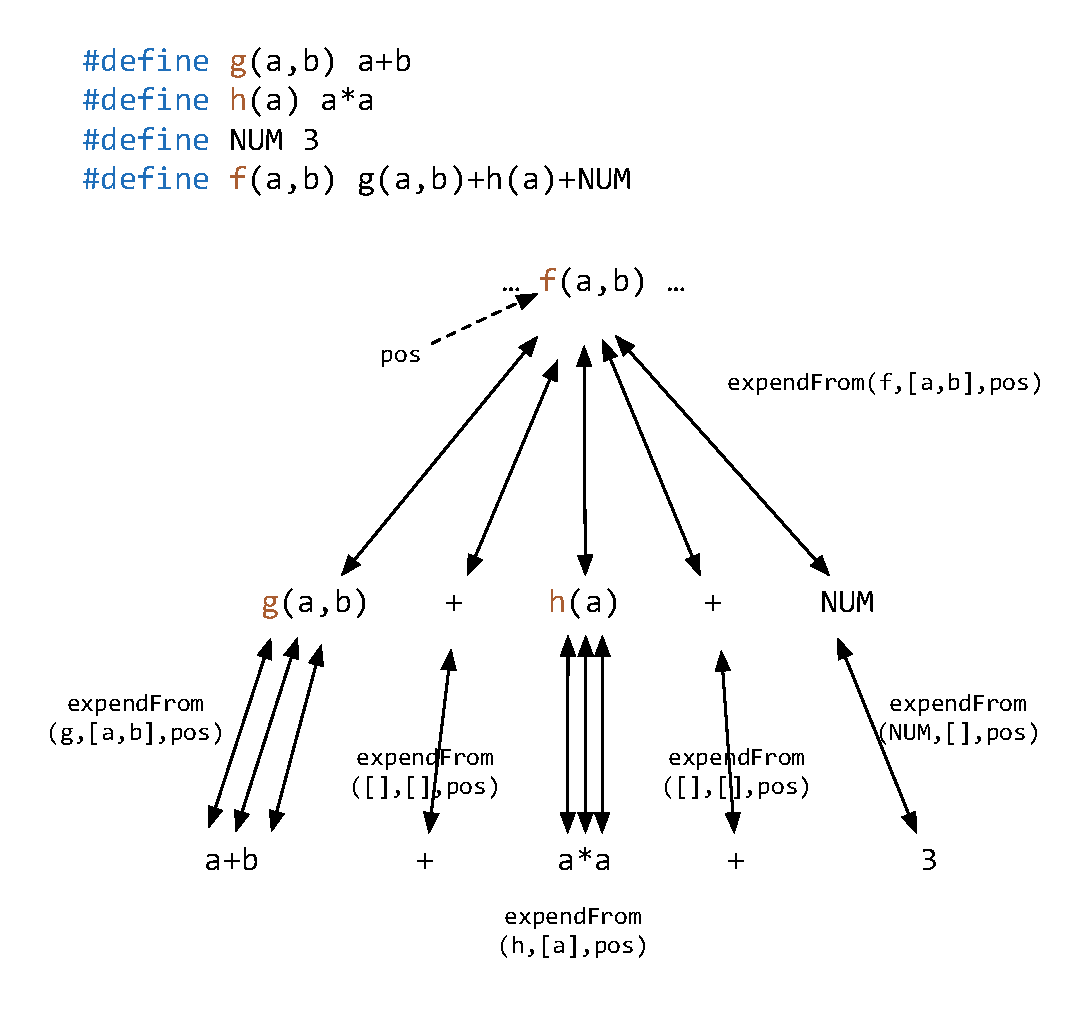
\includegraphics[width=9cm]{pics/original.eps}
\caption{数据结构示例 \label{pic:datastruct}}
\end{figure}

图~\ref{pic:datastruct}展示了宏定义和宏调用展开后的数据结构。构造过程如下:
\begin{itemize}
\item 预处理器扫描源代码发现宏定义指令,将宏定义及其展开式纪录在数据结构中。
\item 当预处理器扫描到位置 $pos$ 时,根据算法规则3,发现函数式宏(\emph{function-like macro})
  调用,分析参数数量,确认宏调用
\item 确认宏调用后,在 $pos$ 位置建立切分点,认为 $f(a, b)$ 是一个独立代码段单元。
  在实现中,这些单元用$Unit$类及其子类实现
\item 独立对$f(a, b)$递归正向展开。正向展开算法在前文中提到(算法~\ref{alg:forward})。
  纪录展开时响应参数位置。
\end{itemize}

图~\ref{pic:datastruct}中的双向箭头表示了词和代码段单元之间的关联关系。
$expandedFrom$中的三个参数表示在下一层的词在正向展开时的来源。
第一个参数描述了该词来源于哪一个宏定义;
第二个参数描述了展开宏时的参数列表,$[]$ 代表空,即没有参数;
第三个参数描述了顶层宏展开在源代码中的位置。
在本例中,第二层中的 $NUM$ 指向第一层的箭头中,$f$ 表示该词被名为 $f$ 的宏展开,
$[a, b]$表示参数列表, $pos$表示展开在源代码中的位置。

我们可以看到,记录下了这些信息和前文提到的重写步骤的信息
可以互换。因此我们就能在这样的数据结构上
应用我们的反向算法,实现双向预处理器。


\subsubsection{BXCPP框架}
我们基于JCPP实现了自己的双向预处理器BXCPP。所有的项目代码和实验数据都可以
在我们的项目网站\footnote{\url{https://github.com/harouwu/BXCPP}}上找到。
在此我们简介一下BXCPP框架中主要的几个类。
\begin{figure}
\centering
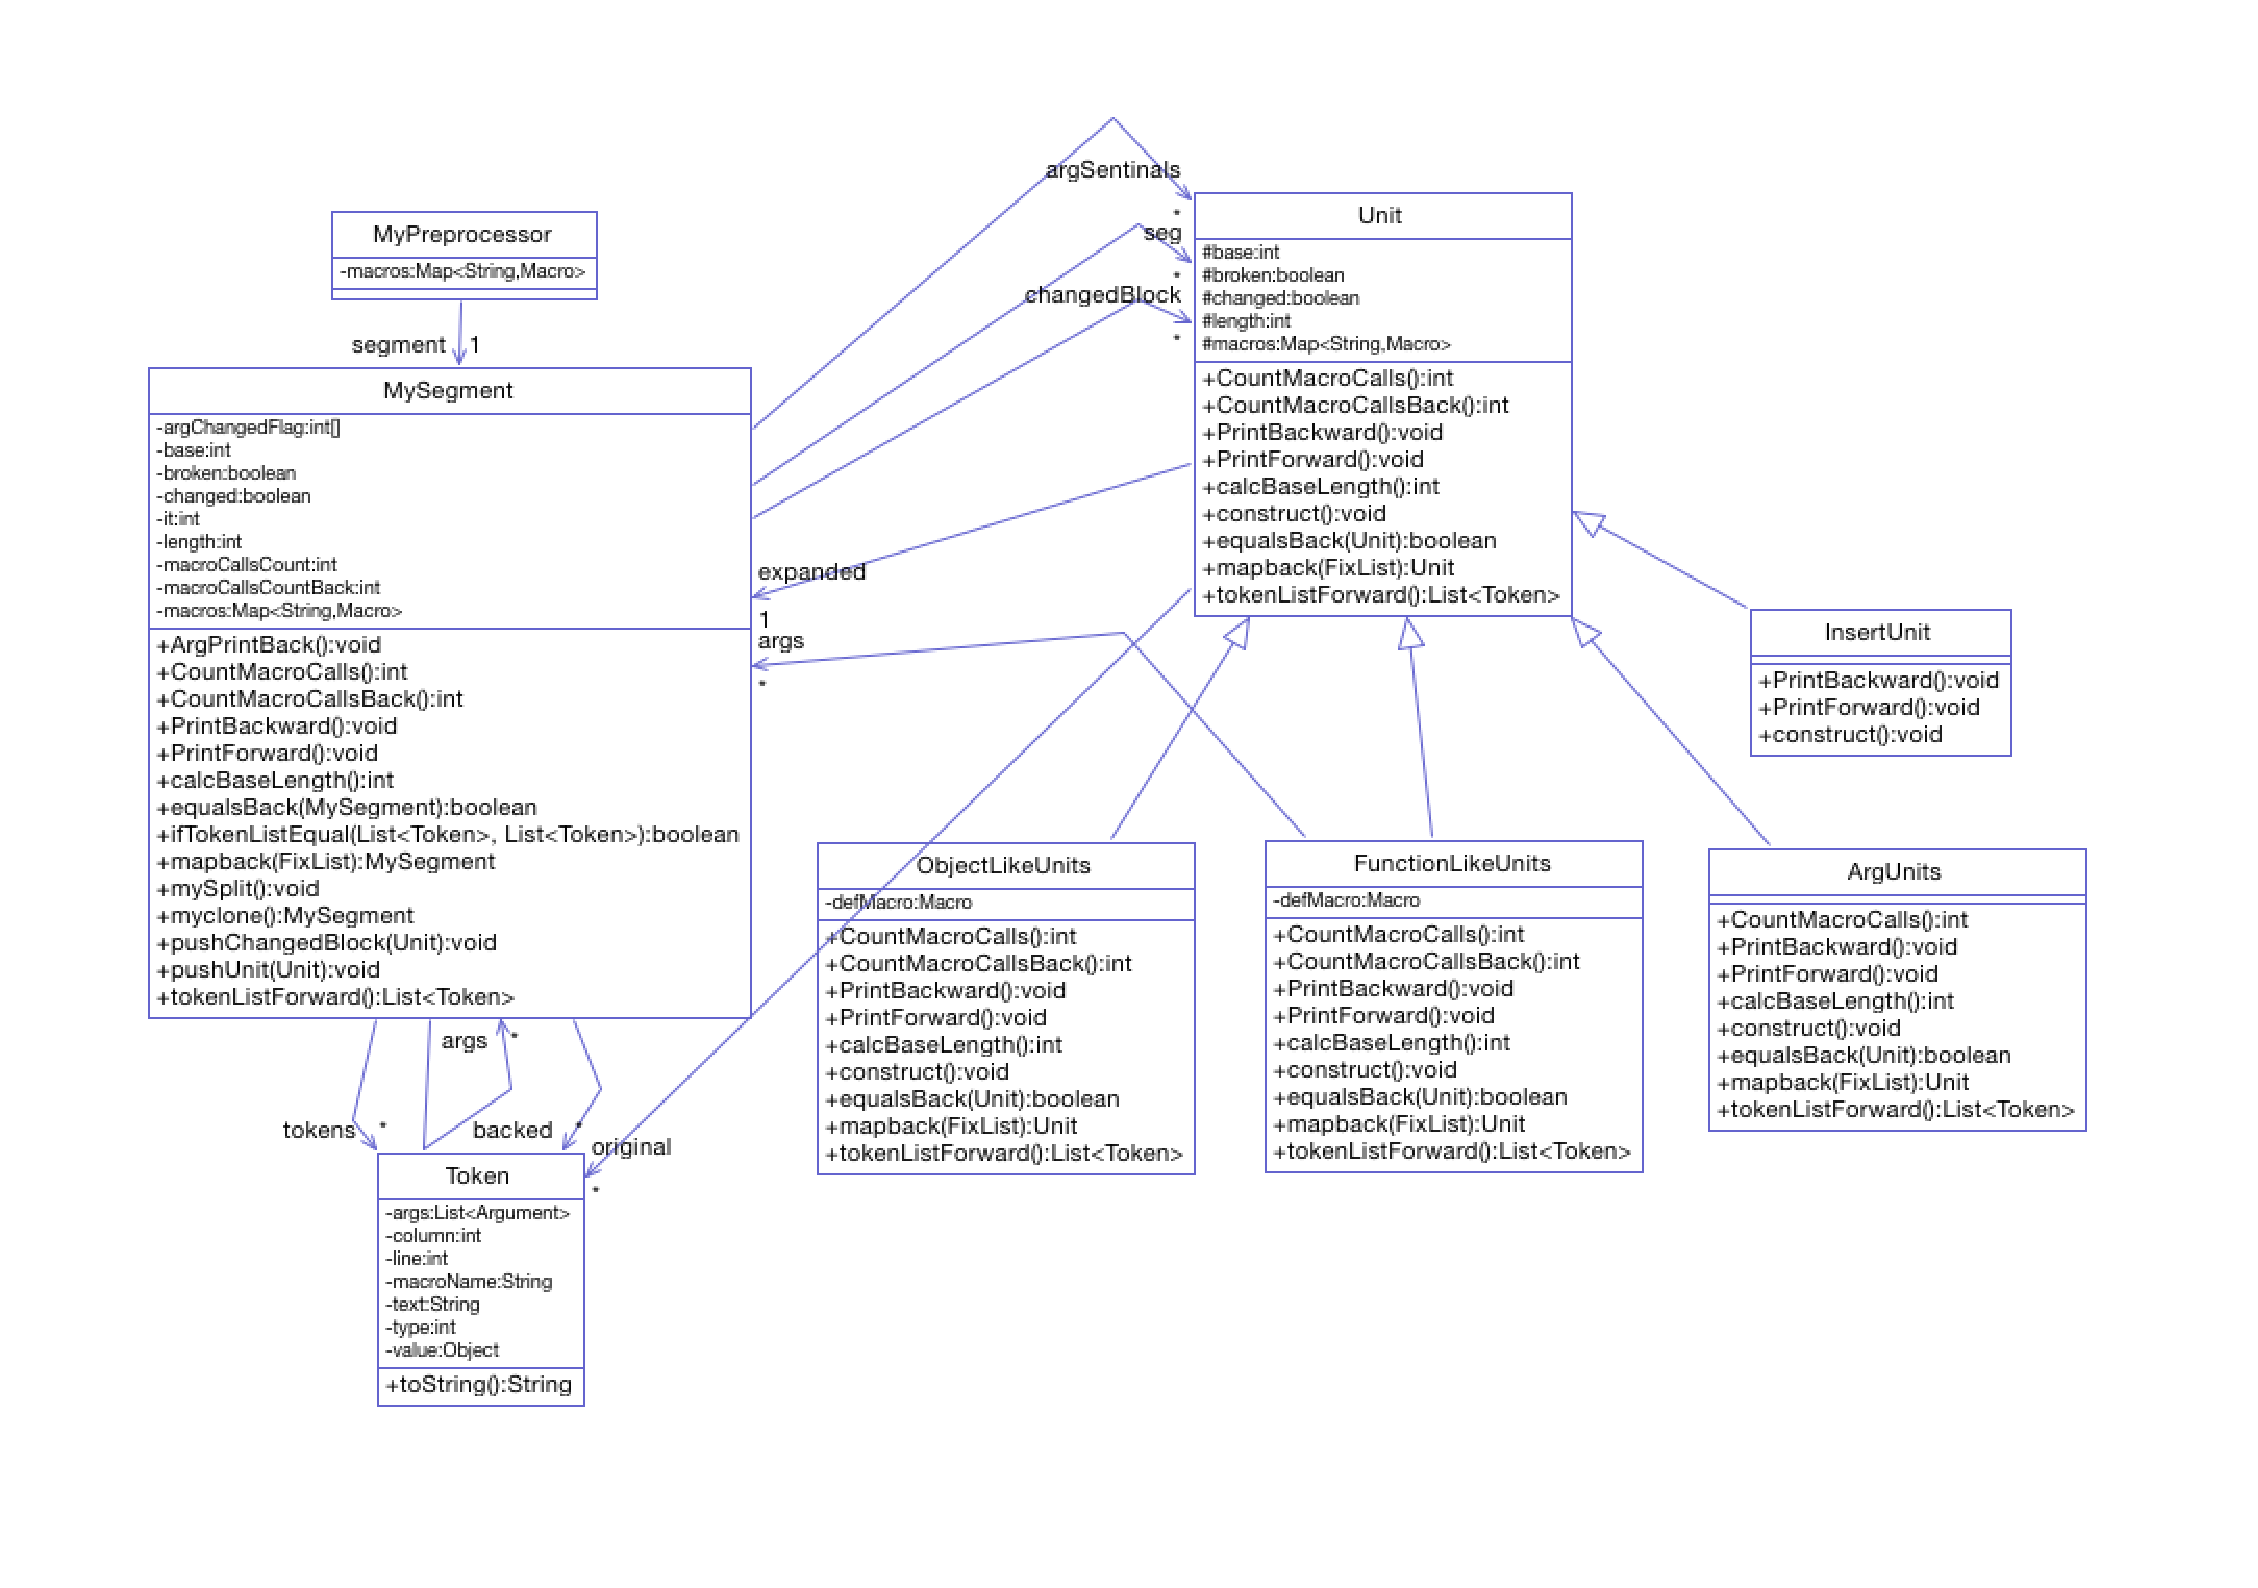
\includegraphics[width=14cm]{pics/class.eps}
\caption{主要类类图。\label{pic:classd}}
\end{figure}


图~\ref{pic:classd}是代码中主要类的类图。小箭头表示包含关系,空心箭头表示继承关系。
我们重写了JCPP中的预处理器 $Preprocessor$类,构造自己的双向C预处理器 $MyPreprocessor$。
该双向预处理器可以识别预处理指令,建立上下文环境纪录和宏定义索引。
同时,双向预处理器把源程序词序列化后,将会把序列保存在类型 $MySegment$里。
$MySegment$封装了词序列和代码段单元序列,同时包含识别拆分代码段单元的函数,类似算法中的$guard$函数。


$Unit$及其子类描述了各种不同类型的代码段单元,他的子类中:
$StringUnit$表示普通文本代码段单元,
$ObjectLikeUnits$表示非函数宏调用代码段单元,
$FunctionLikeUnits$表示函数宏调用代码段单元,
$ArgUnits$表示宏调用参数代码段单元,
$InsertUnit$表示展开式中插入宏参数的代码段单元。

从类图中可以看到,$MySegment$ 和 $Unit$ 类互相包含。
$MySegment$ 中含有 $Unit$ 代码段单元的序列,
而$Unit$在展开时,又包含新的代码段$MySegment$。
这样循环的关系模拟了上一节~\secref{sec:datastruct}中的数据结构,实现了算法。

另外,项目中还定义了许多其他类,如$Token$类描述了词的文本类型等。
具体的项目文档和程序细节,可以访问我们的项目网站了解。
同时我们也实现了前文中提到的 \emph{per-line} 和 \emph{per-file}
两种简单的反向预处理操作。
至此,实现部分基本搭建完成。


\subsubsection{实验基准}
我们的实验在Linux内核版本3.19上执行。我们选择Linux内核源代码因为
Linux是现在最广泛的C语言项目。这之中有许多程序员贡献的代码,包含了不同风格的代码,
也含有大量的预处理指令和宏调用。

为了执行我们的实验,我们需要在Linux内核代码上生成一组修改。
因为我们想看到不同反向预处理算法对程序的影响如何,所以我们需要的修改
应该尽可能出现在有宏调用的函数中。
同时我们在观察中发现,在实际代码中,非函数式宏调用的出现频率
远远高于函数式宏调用。这样导致如果随机生成修改,
大多数修改都会修改非函数式调用,而少数会修改函数式调用。
所以我们根据概率模型,控在非函数式和函数式宏调用的比例为1.5:1。
基于上面的这些计算和宏调用,最终我们从项目中抽取了8000行代码,这之中一共出现了133次宏调用。

接着我们为这抽取的8000行代码生成一组修改。为了模拟现实工程项目中出现的修改,
我们随机性地生成两类修改操作。
第一种是词级别的修改操作,我们随机地替换、删除或插入一个次。
第二种是语句级别的修改,我们随机地删除一句语句、或者从别处随机抽取一句话插入当前位置。
这两种修改的选择是取自现在主流的代码修改工具的方法~\parencite{le2012genprog,QiMLDW14,kim2013automatic}。
其中,GenProg~\parencite{le2012genprog} 和
RSRepair\parencite{QiMLDW14}会直接食用语句级别的修改。
而第一种词级别饿修改则模拟了 PAR~\parencite{kim2013automatic}
中使用的例如替换参数、修改操作符等细微操作。

具体的修改生成过程如下:我们以概率$p$选择在每个词上进行操作。
这个操作可以是插入、替换或删除,三者等概率。
替换操作随机调换一个词中不同字符的位置。
插入操作随机从别处拷贝一个词插入。
类似的,对于每个句子,我们也有味$q$的概率对它生成修改。
修改内容可以是复制或者删除。
复制操作直接把之前一句语句复制过来。
我们根据C语法,根据分号来划分句子。

不同的程序编辑工作会有不同的修改模式:
一个移动工具可能会修改程序中的许多未知,但一个代码修复工具只会修改
程序的少数地方。
为了模拟不同工具之间给出的修改模式,
我们设计了两套不同概率的修改操作集。
一套是高修改密度的操作集合,我们设置$p=0.33$ 和 $q=0.1$。
另一套是低修改密度的操作集合,我们设置$p=0.1$ 和 $q=0.05$。

我们生成了10组修改操作集合,其中5个是高密度的,5个是低密度的。
具体生成的修改数量在表~\ref{tbl:changes}中。
\begin{table}[htbp]
\caption{C实验中生成的修改操作}\label{tbl:changes}
\centering
% \begin{tabular}{|l|lllll|lllll|}
%   \hline
%   Density & \multicolumn{5}{c|}{Low} & \multicolumn{5}{c|}{High} \\
%   \hline
%   Set & 1 & 2& 3& 4 & 5 & 6 & 7 &8 &9 &10\\
%   \hline
%   Changes & 952 & 885 & 956 & 967 & 884 & 3133 & 3136 & 3088 & 3123 &
%                                                                       3048 \\
% \hline
% \end{tabular}
\begin{tabular}{|l|l|lllll|}
  \hline
  \multirow{2}{2cm}{Low Density} & Set & 1 & 2 & 3 & 4 & 5  \\
  \cline{2-7}
                                 & Changes & 952 & 885 & 956 & 967 & 884 \\
  \hline
  \multirow{2}{2cm}{High Density} & Set & 6 & 7 & 8 & 9 & 10 \\
  \cline{2-7}
                                 & Changes & 3133 & 3136 & 3088 & 3123 & 3048\\
  \hline
\end{tabular}
\end{table}

\subsubsection{自变量}
实验中我们认为以下变量是自变量:
(1)\emph{Techniques},我们认为我们的算法和另外两种简单的算法,
per-file和per-line不同。
(2)\emph{修改密度},不同组之间,修改出现的密度不同。我们的实验中同时出现高密度和低密度。

\subsubsection{因变量}
实验中我们认为有两个因变量。
(1)\emph{剩余宏调用的数量}。我们在反向预处理后再次调用正向预处理,
  依次纪录有多少宏调用被展开。因为实验的方法中没有一种会引入新的宏调用,
  所以纪录下的就是剩余宏调用的数量。
  为了减少包含系统头文件中的宏调用带来的干扰,我们只会记录当前文件中的
  宏调用展开次数。
(2)\emph{错误的数量}。这里的错误是指当我们在反向预处理后再次调用正向预处理,
  比较新生成的预处理后代码和之前应用修改的预处理后代码之间是否不同。
  这里我们使用Unix系统提供的文件比较工作 $fc$。
  每当$fc$给出一处不同时,我们认为是一个错误。
(3)\emph{报错}。我们的方法会检测修改能否被映射回去,
我们对于生成的修改操作集合,我们也会记录报错的数量。


\subsection{影响实验可信度的因素}
一个影响实验外部可信度的因素是我们生成的这些修改操作能不能被一般化为
真实项目中产生的程序修改。
为了减轻该因素的影响,我们使用了从现有工具分析得来的不同类型的修改,
同时控制修改出现的频率,这样可以更好地模拟现实项目中的程序修改。

一个影响实验内部可信度的因素是我们实现的三种双向预处理器可能实现错误。
为了减轻该因素的影响,我们通过在Linux内核,自写测试集上不断修改错误来
保证我们的实现是可信可靠的,不会对实验产生负面影响。

\subsection{实验结果}
\begin{table}[htbp]
  \caption{实验结果}\label{tbl:results}
\centering
\begin{tabular}{|l|l|lllll|}
  \hline
  Low Density & Set & 1 & 2 & 3 & 4 & 5\\
  \hline
  \multirow{3}{*}{Our Approach} &  Macros & 73 & 75 & 72 & 80 & 81 \\
  \cline{2-7}
              &Errors & 0 & 0 & 0 & 0 & 0  \\
  \cline{2-7}
              & Failures & n & n & n & n & n \\
  \hline
  \multirow{3}{*}{Per-Line} & Macros & 23 & 25 & 23 & 20 & 26 \\
  \cline{2-7}
              & Errors & 6 & 7 & 6 & 7 & 7  \\
  \hline
  \multirow{3}{*}{Per-File} & Macros & 0 & 0 & 0 & 0 & 0  \\
  \cline{2-7}
              & Errors & 0 & 0 & 0 & 0 & 0 \\
  \hline
  \hline
  High Density & Set & 6 & 7 & 8& 9& 10\\
  \hline
  \multirow{3}{*}{Our Approach} &Macros & 47 & 51 & 53 & 48 & 44 \\
  \cline{2-7}
              &  Errors & 0 & 0 & 0 & 0 & 0  \\
  \cline{2-7}
              & Failures & n & n & n & n & n \\
  \hline
  \multirow{3}{*}{Per-Line} & Macros & 9 & 7 & 7 & 8 & 10  \\
  \cline{2-7}
              & Errors & 6 & 6 & 7 & 6 & 6 \\
  \hline
  \multirow{3}{*}{Per-File} & Macros & 0 & 0 & 0 & 0 & 0  \\
  \cline{2-7}
              & Errors & 0 & 0 & 0 & 0 & 0 \\
  \hline\end{tabular}
\\
\parbox{\columnwidth}{ \ \\
\footnotesize ``Macros'' 行表示剩余的宏调用数量。``Errors'' 行表示修改造成的错误数量
      ``Failure'' 行表示反向预处理器发生了多少错误。}
\end{table}

% \begin{table*}[htbp]
% \caption{Macros remainings and errors of different algorithms and data set}
% \centering
% \begin{tabular}{l|cc|cc|cc}
% \hline
% Algorithm  &High Mutation & &Low Mutation & &Average &  \\
%  &Remain &Error &Remain &Error &Remain &Error \\
% \hline
% CPP-TRANS &120 &0 &243.8 &0 &181.9 &0 \\
% PER-FILE &0 &0 &0 &0 &0 &0  \\
% PER-LINE &25.6 &5.8 &64.2 &2.4 &44.9 &4.1 \\
% \hline
% \end{tabular}
% \end{table*}

我们实验的结果在表~\ref{tbl:results}中。
接着我们将会讨论本章开始时提到的三个研究问题的解答。 

\subsubsection{研究问题1} 我们从表中可以看出,我们的方法尽可能地保存了宏调用。 
Per-line方法保留了一些宏调用,而per-file方法,不出所料的,完全不
保留宏调用。我们进一步考察了为什么per-line方法保存了这么少的宏调用。
其中一个主要原因是我们发现在Linux内核代码中,时常出现一行中有多个宏调用
的情况。而一旦修改发生在该行,
per-line方法会破坏该行中的所有宏调用。
\subsubsection{研究问题2} 从表中看出,我们的方法和per-file方法都不会产生错误。
但per-line方法产生了一些错误。我们认为这是因为存在一些宏调用形式是多行
宏调用。这些宏调用的参数一般是一个表达式,甚至一个句子,以至于一行中
无法写完而需要换行。
\subsubsection{研究问题3} 正如之前讨论过的,我们的方法会在反向变换时对
不合适的修改操作进行报错。这是因为有时一个修改会意外地在预处理后的代码中引入一个新的宏调用。
这样就无法满足正确性性质的PUTGET性质。
但是,在我们的实验中没有看到类似的情况。
这是因为宏定义的名字之间差别比较大,而宏调用的位置在整个代码中很零散,通过调换字符位置或者拷贝
并不能引入不合适的修改操作。
同时我们知道另外两种方法并不能检测这种不合适的修改操作,
所以在表~\ref{tbl:results}关于报错的部分都留空了。

尽管出现不合适的修改操作而导致报错的情况在实际工作中也不常见,
但理论上我们的方式是可以对这种情况作出报错的。

%另外理论上我们的方式可以能会出现误报情况:
%我们的算法报错但是存在一种映射修改的方式。
%比方说我们考虑以下代码:
%\begin{lstlisting}
%#define p (x)
%plus p
%\end{lstlisting}
%$plus$是在之前的代码段~\eqref{eqn:expansion}中定义的宏。
%在预处理后这段代码会展开成$plus\ (x)$。
%如果我们把最后的括号拆分成$)\ hello$,那么这个修改会使得我们的方法报错

%Although probably being rare in practice, theoretically our approach
%may report false alarms: our approach reports a failure but
%a correct change on the source program exists. {For example, let consider the
%  following code piece,
%\begin{lstlisting}
%#define p (x)
%plus p
%\end{lstlisting}
%where $plus$ is the macro defined in code
%piece~\eqref{eqn:expansion}. After preprocessing, this code piece becomes
%$plus\ (x)$. If we change the last parenthesis into $)\ hello$, our
%approach reports a failure because first $p$ will be expanded and then
%the expanded content forms a new macro invocation with $plus$.
%However, there exists a feasible change: replacing $p$ with $hello\ p$.}
%\end{comment}

%%% Local Variables:
%%% mode: latex
%%% TeX-master: "main"
%%% End:

\chapter{相关工作}
\section{Related Work}
\label{sec:related}

\subsection{双向变换领域}
我们工作的灵感来自于双向变换领域的研究。
双向变换领域中一个经典的使用情况就是数据库设计中的
\emph{view-update problem}~\parencite{BaSp81,DaBe82,Hegner90,Cui2000,Fegaras2010}:
一个域表示一个为一条查询指令计算好的数据库,
研究工作主要关注于如何把在这个域上做的修改操作反向升级到源数据库中。
这个工作就像\emph{模块转化}在软件进化中一样重要~\parencite{YuLHHKM12,XiLHZTM07}。

同时,针对这种双向变换的应用,学术界也设计了许多语言使得工作更加方便。
其中广为人知晓的是 \emph{透镜}理论框架~\parencite{HuMT04,MuHT04aplas,Foster:2007,BoFPPS08,FoPP08,WaGMH10,Diskin2011,Hofmann2012,FoMV12,RaLFC13}。
在这套框架下涵盖了许多为双向变换提供连接因子的语言架构。
另一种比较主流的思想是自动化地为现存的非双向变换的程序
找到对应的反向程序。这类的研究称为 \emph{双向变换化(Bidirectionalization)}
~\parencite{MaHNHT07,Voigtlander09bff,voigtlander2010combining,WaGW11,VoHMW13,WaGMH13,MaWa13,MaWa13ppdp,WaNa14,MaWa14}。
在软件工程的模块转换领域,需要被转换的数据通常以图(并非是树)的结构来保存。
此时主流会使用一个关系型,而非函数型,的方法来描述不同模块之间的双向的不同的关系
~\parencite{qvt,Stevens2010,Schurr1994,Schurr2008,HiHIKMN10,Hidaka:2011}。
但是,我们工作的要求现在并没有一种双向变换的技术可以满足。这是因为在我们的模型中,
不仅作为数据的代码会出现变化,作为转换程序本身的宏、预处理指令,也会有相应的变化。
因此,我们也为这类数据和转换程序都会变化的双向变换模型,提出了自己见解。


\subsection{分析和修改未预处理的C代码}
C的预处理器给静态程序分析带来了巨大的挑战。
由于C的预处理器支持预处理变量,导致分析时,场景数量组合型快速增长。
这使得传统的每次只处理一个变量的程序分析方法变得不可行。
也仅直到最近,通过\emph{family-based
analyses}~\parencite{Kastner2011,Gazzillo2012,Liebig2013}
的方法才能对未预处理的C代码进行可靠的解析与分析。
之前的许多工具都时常出现不可靠的操作,
或者只能限制在非常严格的使用情况下使用~\parencite{Baxter2001,Garrido2005,Padioleau2009}。

类似的,为了处理这种多变量的情况,在C代码重构的研究中学术界也花了很多功夫。
大多数方法~\parencite{Garrido2002,Vittek2003,Spinellis2003,Garrido2013}都试图
找到一个能够同时表示C语法和预处理器指令的合适模型。
最近有一项工作~\parencite{Overbey2014}提出了另外一种方法:
为某一个变量做重构,但如果这对其他变量产生影响就阻止重构。
这项工作是基于预处理变量修改相互之间往往影响很小的观测而设计出来的。
我们可以看到,解决预处理前代码的分析现在并没有优秀的解决方案。

需要承认的是,我们的项目现在暂时也只考虑一个变量。
在未来我们可能会把我们的工作和多变量的算法相结合。
但是,即使只能处理一个变量,我们的项目在许多方面都十分有用:
(1)许多实际工作中的程序,尽管有许多条件编译选项,没有许多预处理变量。
(2)Overbey等人~\parencite{Overbey2014}在他们的论文中指出,
现实中修改一个变量往往不会对其他变量造成影响。
%  However, our approach requires minimal
% changes to existing tools, so can potentially be applied to many areas
% that do not require specialized effort.

% Refactoring unpreprocessed C code is extremely difficult. Even without considering the above mentioned problem with parsing, dealing with macro expansion while editing remains tricky~\cite{Garrido2002,Vittek2003,Spinellis2003,Garrido2013,Overbey2014}. Even for relatively simple tasks such as identifying and removing dead code sophisticated analyses are required~\cite{Baxter2001,Tartler2011}. 

% Our proposal in this paper does not apply to the cases here. We do
% not consider multiple configurations, and we do not allow explicit
% modification of preprocessor directives.

% Though our approach is able to handle some refactorings, our approach
% cannot replace these approaches because (1) as discussed before, our
% approach do not consider multiple configurations, and (2) our approach
% does not change preprocessor directives, which is necessary in
% refactorings such as renaming macros and extract macros.

%Work by Christian Kastner
%
%Parsing C/C++ code without pre-processing by Y Padioleau, CC'09
%
%SuperC: parsing all of C by taming the preprocessor, PLDI'12

\subsection{C预处理器上的实例调查}
许多年来,学术界不乏各类对C预处理器十分有见解的学术实例调查工作
~\parencite{Spencer92,ernst2002empirical,Liebig2011}。
同时也有一些C预处理的替代品被提出,比如语法预处理器~\parencite{Weise1993,McCloskey:2005}
或者面向侧面开发方法~\parencite{Lohmann2006,Adams2009,Boucher2010}。
但是直至今日,业界并没有什么采用这类替代预处理器的迹象,
C预处理器依然是主流的工具。
这也说明C预处理器带来的麻烦依然广泛存在。



%%% Local Variables: 
%%% mode: latex
%%% TeX-master: "main"
%%% End: 

\chapter{总结}
\label{sec:conclusion}

为程序编辑工具处理C预处理器十分困难。
现有的程序编辑工具往往无法正确处理预处理指令、或是直接不处理预处理指令。
例如现有的C语言工具:GenProg~\parencite{le2012genprog,le2012systematic},RSRepair~\parencite{QiMLDW14},和
SemFix~\parencite{nguyen2013semfix}。
这三个工具都只在预处理后的代码上工作。

本文中我们使用双向变换的方法提出了一种轻量级的双向C预处理器。
我们模拟了正向C预处理器算法,并将其转化到重写规则模型中。
我们根据重写规则模型定义了重写步骤数据结构。
我们依据重写步骤结构生成反向变换,并讨论了该双向预处理过程是否满足应有的5条性质。

另外,我们在Linux内核上验证了我们的方法,并和另外两种基本的
做法进行比较。
实验的结果显示相较于其他方法,我们的方法破坏了相当少的宏调用,
并且总是可以给出正确的修改,而其他方法有时不行。

总的说来,该方法把程序编辑工具从预处理器带来的设计麻烦中解脱出来。
使得程序编辑工具能专注于预处理之后的代码,达到更模块化的设计效果。
这是已知的第一种双向预处理器。

从理论上说,C预处理器涉及到的问题也可以看作是转换系统问题中特殊的一类。
在这类问题中,转换程序和数据可能同时被转换。
例如双向变换PHP设计~\parencite{wang2012automating}。
现有的方法~\parencite{wang2012automating}往往使用十分复杂且有针对性的设计。
其中关于双向变换性质的定义和正确性的讨论也往往很复杂。
本文所提出的方法对这一类的问题都有适用价值:该方法把转换程序当作数据,
并在更高一层的操作语义上生成双向变换。
我们衷心希望未来能看到更通用的理论能够完美解决这一类问题。



%%% Local Variables: 
%%% mode: latex
%%% TeX-master: "main"
%%% End: 


\section*{Acknowledge}
We would like to acknowledge Yangyi Wu at Peking University for the
fruitful discussions during the early stage of this work.

\bibliographystyle{IEEEtran}
\bibliography{reference,main}

\end{document}

%%% Local Variables:
%%% mode: latex
%%% TeX-master: t
%%% End:
